\documentclass{article}[10pt]
\usepackage{array}
\usepackage{mathtools}
\usepackage{amsfonts}
\usepackage{tikz}
\usepackage{amsmath}
\usepackage{kotex}
\usepackage{multirow}

\usetikzlibrary{arrows}
\tikzset{
  treenode/.style = {align=center, inner sep=0pt, text centered},
  arn/.style = {treenode, circle, black, draw=black, text width=0.6cm, line width=0.25mm},
  arn_u/.style = {treenode, circle, black, draw=white, text width=0.6cm, line width=0.25mm},
}

\newcommand{\inbox}[1]{\begin{tabular}{|>{\centering}m{1.0\textwidth}|}\hline \\
#1 \\ \end{tabular}}

\begin{document}

\inbox{
\begin{tabular}{c@{\hskip3em}c@{\hskip3em}c}


\begin{tikzpicture}[level/.style={sibling distance = 1.5cm/#1, level distance = 1cm}]
  \node [arn] {};
\end{tikzpicture}

  &

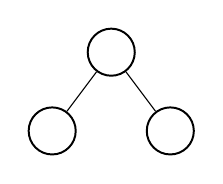
\begin{tikzpicture}[level/.style={sibling distance = 1.5cm/#1, level distance = 1cm}]
  \node [arn] {}
  child{
    node [arn] {}
  }
  child{
    node [arn] {}
  };
\end{tikzpicture}

  &

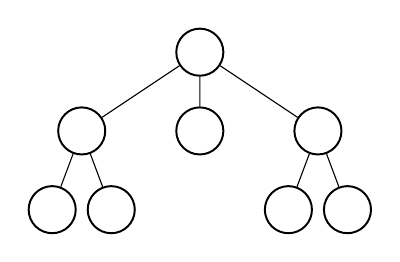
\begin{tikzpicture}[level/.style={sibling distance = 1.5cm/#1, level distance = 1cm}]
  \node [arn] {}
  child{
    node [arn] {}
    child{
      node [arn] {}
    }
    child{
      node [arn] {}
    }
  }
  child{
    node [arn] {}
  }
  child{
    node [arn] {}
    child{
      node [arn] {}
    }
    child{
      node [arn] {}
    }
  };
\end{tikzpicture}

\\

  나무 1 & 나무 2 & 나무 3 \\

\end{tabular}
}

\inbox{
\begin{tabular}{c@{\hskip3em}c@{\hskip3em}c}


\begin{tikzpicture}[level/.style={sibling distance = 1.5cm/#1, level distance = 1cm}]
  \node [arn] {1};
\end{tikzpicture}

  &

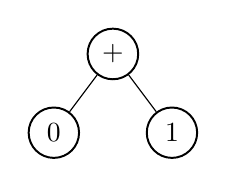
\begin{tikzpicture}[level/.style={sibling distance = 1.5cm/#1, level distance = 1cm}]
  \node [arn] {+}
  child{
    node [arn] {0}
  }
  child{
    node [arn] {1}
  };
\end{tikzpicture}

  &

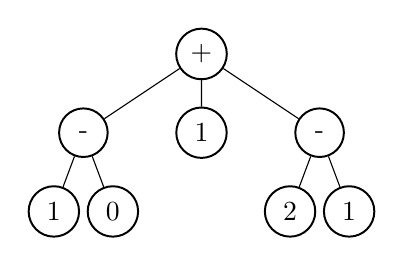
\begin{tikzpicture}[level/.style={sibling distance = 1.5cm/#1, level distance = 1cm}]
  \node [arn] {+}
  child{
    node [arn] {-}
    child{
      node [arn] {1}
    }
    child{
      node [arn] {0}
    }
  }
  child{
    node [arn] {1}
  }
  child{
    node [arn] {-}
    child{
      node [arn] {2}
    }
    child{
      node [arn] {1}
    }
  };
\end{tikzpicture}

\\

  나무 1$'$ & 나무 2$'$ & 나무 3$'$ \\

\end{tabular}
}

\inbox{
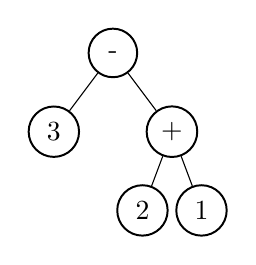
\begin{tikzpicture}[level/.style={sibling distance = 1.5cm/#1, level distance = 1cm}]
  \node [arn] {-}
  child{
    node [arn] {3}
  }
  child{
    node [arn] {+}
    child{
      node [arn] {2}
    }
    child{
      node [arn] {1}
    }
  };
\end{tikzpicture}
}

\inbox{
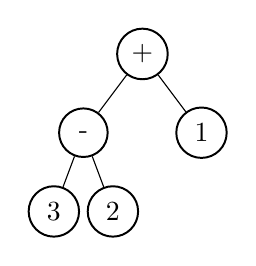
\begin{tikzpicture}[level/.style={sibling distance = 1.5cm/#1, level distance = 1cm}]
  \node [arn] {+}
  child{
    node [arn] {-}
    child{
      node [arn] {3}
    }
    child{
      node [arn] {2}
    }
  }
  child{
    node [arn] {1}
  };
\end{tikzpicture}
}

\inbox{
  \begin{tabular}{>{\raggedleft}m{0.2\textwidth}>{\centering}m{0.2\textwidth}m{0.2\textwidth}}
  $n\in\mathbb{Z}$이면, &
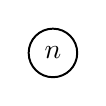
\begin{tikzpicture}[level/.style={sibling distance = 1.5cm/#1, level distance = 1cm}]
  \node [arn] {$n$};
\end{tikzpicture}
  & $\in E$ \\
  $e_1,e_2\in E$이면, &
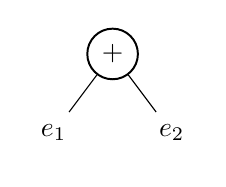
\begin{tikzpicture}[level/.style={sibling distance = 1.5cm/#1, level distance = 1cm}]
  \node [arn] {$\mathsf{+}$}
  child{
    node [arn_u] {$e_1$}
  }
  child{
    node [arn_u] {$e_2$}
  };
\end{tikzpicture}
  & $\in E$ \\
  $e_1,e_2\in E$이면, &
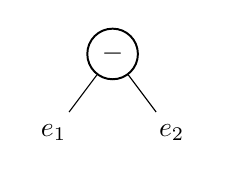
\begin{tikzpicture}[level/.style={sibling distance = 1.5cm/#1, level distance = 1cm}]
  \node [arn] {$\mathsf{-}$}
  child{
    node [arn_u] {$e_1$}
  }
  child{
    node [arn_u] {$e_2$}
  };
\end{tikzpicture}
  & $\in E$ \\
\end{tabular}
}

\inbox{
\begin{tabular}{>{\raggedleft}m{0.2\textwidth}>{\centering}m{0.2\textwidth}m{0.2\textwidth}}
  $n\in\mathbb{Z}$이면, &
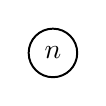
\begin{tikzpicture}[level/.style={sibling distance = 1.5cm/#1, level distance = 1cm}]
  \node [arn] {$n$};
\end{tikzpicture}
  & $\in E$ \\
\end{tabular}
}

\inbox{
\begin{tabular}{>{\raggedleft}m{0.2\textwidth}>{\centering}m{0.2\textwidth}m{0.2\textwidth}}
  $e_1,e_2\in E$이면, &
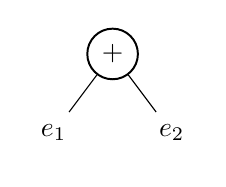
\begin{tikzpicture}[level/.style={sibling distance = 1.5cm/#1, level distance = 1cm}]
  \node [arn] {$\mathsf{+}$}
  child{
    node [arn_u] {$e_1$}
  }
  child{
    node [arn_u] {$e_2$}
  };
\end{tikzpicture}
  & $\in E$ \\
\end{tabular}
}

\inbox{
\begin{tabular}{>{\raggedleft}m{0.2\textwidth}>{\centering}m{0.2\textwidth}m{0.2\textwidth}}
  $e_1,e_2\in E$이면, &
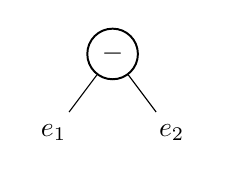
\begin{tikzpicture}[level/.style={sibling distance = 1.5cm/#1, level distance = 1cm}]
  \node [arn] {$\mathsf{-}$}
  child{
    node [arn_u] {$e_1$}
  }
  child{
    node [arn_u] {$e_2$}
  };
\end{tikzpicture}
  & $\in E$ \\
\end{tabular}
}

\inbox{
  \begin{tabular}{>{\raggedleft}m{0.2\textwidth}>{\centering}m{0.2\textwidth}m{0.2\textwidth}}
  $n\in\mathbb{Z}$이면, &
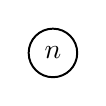
\begin{tikzpicture}[level/.style={sibling distance = 1.5cm/#1, level distance = 1cm}]
  \node [arn] {$n$};
\end{tikzpicture}
  & $\in E'$ \\
  $e_1,e_2\in E'$이면, &
\begin{tikzpicture}[level/.style={sibling distance = 1.5cm/#1, level distance = 1cm}]
  \node [arn] {\scriptsize 덧셈}
  child{
    node [arn_u] {$e_1$}
  }
  child{
    node [arn_u] {$e_2$}
  };
\end{tikzpicture}
  & $\in E'$ \\
  $e_1,e_2\in E'$이면, &
\begin{tikzpicture}[level/.style={sibling distance = 1.5cm/#1, level distance = 1cm}]
  \node [arn] {\scriptsize 뺄셈}
  child{
    node [arn_u] {$e_1$}
  }
  child{
    node [arn_u] {$e_2$}
  };
\end{tikzpicture}
  & $\in E'$ \\
\end{tabular}
}

\inbox{
\begin{tabular}{c@{\hskip3em}c}


\begin{tikzpicture}[level/.style={sibling distance = 1.5cm/#1, level distance = 1cm}]
  \node [arn] {1};
\end{tikzpicture}

  &

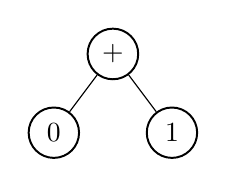
\begin{tikzpicture}[level/.style={sibling distance = 1.5cm/#1, level distance = 1cm}]
  \node [arn] {+}
  child{
    node [arn] {0}
  }
  child{
    node [arn] {1}
  };
\end{tikzpicture}

\\

  나무 1$'$ & 나무 2$'$ \\

\end{tabular}
}

\end{document}
